\documentclass[a4paper, 12pt]{article}

%------Lang
\usepackage[french]{babel}

%------base
%------------------------------------------------------------------------
% This is a LaTeX template, with some useful commands and environments.
%
% Author                :   Lasercata
% Last modification     :   2023.12.18
% Version               :   v6.0.4
%
%------------------------------------------------------------------------


%------ini
\usepackage[utf8]{inputenc}
\usepackage[T1]{fontenc}


%------geometry
\usepackage[textheight=700pt, textwidth=470pt]{geometry}


%------color
\usepackage{xcolor}
\definecolor{ff4500}{HTML}{ff4500}
\definecolor{00f}{HTML}{0000ff}
\definecolor{0ff}{HTML}{00ffff}
\definecolor{656565}{HTML}{656565}

\newcommand{\Emph}{\textcolor{ff4500}}

\newcommand{\strong}[1]{\textcolor{ff4500}{\bf #1}}
\newcommand{\st}{\color{ff4500}\bf}


%------Code highlighting
%---listings
\usepackage{listings}

\definecolor{cbg}{HTML}{272822}
\definecolor{cfg}{HTML}{ececec}
\definecolor{ccomment}{HTML}{686c58}
\definecolor{ckw}{HTML}{f92672}
\definecolor{cstring}{HTML}{e6db72}
\definecolor{cstringlight}{HTML}{98980f}
\definecolor{lightwhite}{HTML}{fafafa}

\lstdefinestyle{DarkCodeStyle}{
    backgroundcolor=\color{cbg},
    commentstyle=\itshape\color{ccomment},
    keywordstyle=\color{ckw},
    numberstyle=\tiny\color{cbg},
    stringstyle=\color{cstring},
    basicstyle=\ttfamily\footnotesize\color{cfg},
    breakatwhitespace=false,
    breaklines=true,
    captionpos=b,
    keepspaces=true,
    numbers=left,
    numbersep=5pt,
    showspaces=false,
    showstringspaces=false,
    showtabs=false,
    tabsize=4,
    xleftmargin=\leftskip
}

\lstdefinestyle{LightCodeStyle}{
    backgroundcolor=\color{lightwhite},
    commentstyle=\itshape\color{ccomment},
    keywordstyle=\color{ckw},
    numberstyle=\tiny\color{cbg},
    stringstyle=\color{cstringlight},
    basicstyle=\ttfamily\footnotesize\color{cbg},
    breakatwhitespace=false,
    breaklines=true,
    captionpos=b,
    keepspaces=true,
    numbers=left,
    numbersep=10pt,
    showspaces=false,
    showstringspaces=false,
    showtabs=false,
    tabsize=4,
    frame=L,
    xleftmargin=\leftskip
}

%\lstset{style=DarkCodeStyle}
\lstset{style=LightCodeStyle}
%Usage : \begin{lstlisting}[language=Caml, xleftmargin=xpt] ... \end{lstlisting}


%---Algorithm
\usepackage[linesnumbered,ruled,vlined]{algorithm2e}
\SetKwInput{KwInput}{Input}
\SetKwInput{KwOutput}{Output}

\SetKwProg{Fn}{Function}{:}{}
\SetKwProg{Proc}{Procedure}{:}{}
\SetKw{KwPrint}{Print}

\newcommand\commfont[1]{\textit{\texttt{\textcolor{656565}{#1}}}}
\SetCommentSty{commfont}
\SetProgSty{texttt}
\SetArgSty{textnormal}
\SetFuncArgSty{textnormal}
%\SetProgArgSty{texttt}

\newenvironment{indalgo}[2][H]{
    \begin{algoBox}
        \begin{algorithm}[#1]
            \caption{#2}
}
{
        \end{algorithm}
    \end{algoBox}
}


%---tcolorbox
\usepackage[many]{tcolorbox}

\DeclareTColorBox{emphBox}{O{black}O{lightwhite}}{
    breakable,
    outer arc=0pt,
    arc=0pt,
    top=0pt,
    toprule=-.5pt,
    right=0pt,
    rightrule=-.5pt,
    bottom=0pt,
    bottomrule=-.5pt,
    colframe=#1,
    colback=#2,
    enlarge left by=10pt,
    width=\linewidth-\leftskip-10pt,
}

\DeclareTColorBox{algoBox}{O{black}O{lightwhite}}{
    breakable,
    arc=0pt,
    top=0pt,
    toprule=-.5pt,
    right=0pt,
    rightrule=-.5pt,
    bottom=0pt,
    bottomrule=-.5pt,
    left=0pt,
    leftrule=-.5pt,
    colframe=#1,
    colback=#2,
    width=\linewidth-\leftskip-10pt,
}


%-------make the table of content clickable
\usepackage{hyperref}
\hypersetup{
    colorlinks,
    citecolor=black,
    filecolor=black,
    linkcolor=black,
    urlcolor=black
}


%------pictures
\usepackage{graphicx}
%\usepackage{wrapfig}

\usepackage{tikz}

\usepackage{float} % For [H] in figure env


%------tabular
%\usepackage{color}
%\usepackage{colortbl}
%\usepackage{multirow}


%------Physics
%---Packages
%\usepackage[version=4]{mhchem} %$\ce{NO4^2-}$

%---Commands
\newcommand{\link}[2]{\mathrm{#1} \! - \! \mathrm{#2}}
\newcommand{\pt}[1]{\cdot 10^{#1}} % Power of ten
\newcommand{\dt}[2][t]{\dfrac{\mathrm d #2}{\mathrm d #1}} % Derivative
\renewcommand{\d}{\mathrm d}

\newcommand{\rot}{\vect{\mathrm{rot}}}
\newcommand{\grad}{\vect{\mathrm{grad}}}
\renewcommand{\div}{\mathrm{div}}
\renewcommand{\j}{\vec\jmath}


%------math
%---Packages
%\usepackage{textcomp}
%\usepackage{amsmath}
\usepackage{amssymb}
\usepackage{mathtools} % For abs
\usepackage{stmaryrd} %for \llbracket and \rrbracket
\usepackage{mathrsfs} %for \mathscr{x} (different from \mathcal{x})
\usepackage{esint} % Better integrals (double, triple, \oiint, ...)

%---Commands
%-Sets
\newcommand{\N}{\mathbb{N}} %set N
\newcommand{\Z}{\mathbb{Z}} %set Z
\newcommand{\Q}{\mathbb{Q}} %set Q
\newcommand{\R}{\mathbb{R}} %set R
\newcommand{\C}{\mathbb{C}} %set C
\newcommand{\U}{\mathbb{U}} %set U
\newcommand{\seg}[2]{\left[ #1\ ;\ #2 \right]}
\newcommand{\nset}[2]{\left\llbracket #1\ ;\ #2 \right\rrbracket}

%-Exponantial / complexs
\newcommand{\e}{\mathrm{e}}
\newcommand{\cj}[1]{\overline{#1}} %overline for the conjugate.

%-Vectors
\newcommand{\vect}{\overrightarrow}
\newcommand{\veco}[3]{\displaystyle \vect{#1}\binom{#2}{#3}} %vector + coord

%-Limits
\newcommand{\lm}[2][{}]{\lim\limits_{\substack{#2 \\ #1}}} %$\lm{x \to a} f$ or $\lm[x < a]{x \to a} f$
\newcommand{\Lm}[3][{}]{\lm[#1]{#2} \left( #3 \right)} %$\Lm{x \to a}{f}$ or $\Lm[x < a]{x \to a}{f}$
\newcommand{\tendsto}[1]{\xrightarrow[#1]{}}

%-Integral
\newcommand{\dint}[4][x]{\displaystyle \int_{#2}^{#3} #4 \mathrm{d} #1} %$\dint{a}{b}{f(x)}$ or $\dint[t]{a}{b}{f(t)}$

%-left right
\newcommand{\lr}[1]{\left( #1 \right)}
\newcommand{\lrb}[1]{\left[ #1 \right]}
\newcommand{\lrbb}[1]{\left\llbracket #1 \right\rrbracket}
\newcommand{\set}[1]{\left\{ #1 \right\}}
\newcommand{\abs}[1]{\left\lvert #1 \right\rvert}
\newcommand{\norm}[1]{\left\lVert #1 \right\rVert}
\newcommand{\ceil}[1]{\left\lceil #1 \right\rceil}
\newcommand{\floor}[1]{\left\lfloor #1 \right\rfloor}
\newcommand{\lrangle}[1]{\left\langle #1 \right\rangle}

%-Boxes
\newcommand{\oboxed}[1]{\textcolor{ff4500}{\boxed{\textcolor{black}{#1}}}} %orange boxed

\newcommand{\rboxed}[1]{\begin{array}{|c} \hline #1 \\ \hline \end{array}} %boxed with right opened
\newcommand{\lboxed}[1]{\begin{array}{c|} \hline #1 \\ \hline \end{array}} %boxed with left opened

\newcommand{\orboxed}[1]{\textcolor{ff4500}{\rboxed{\textcolor{black}{#1}}}} %orange right boxed
\newcommand{\olboxed}[1]{\textcolor{ff4500}{\lboxed{\textcolor{black}{#1}}}} %orange left boxed

%-Others
\newcommand{\para}{/\!/} %//
\newcommand{\ssi}{\ \Leftrightarrow \ }
\newcommand{\eqsys}[2]{\begin{cases} #1 \\ #2 \end{cases}}

\newcommand{\med}[2]{\mathrm{med} \left[ #1\ ;\ #2 \right]}  %$\med{A}{B} -> med[A ; B]$
\newcommand{\Circ}[2]{\mathscr{C}_{#1, #2}}

\renewcommand{\le}{\leqslant}
\renewcommand{\ge}{\geqslant}


%------commands
%---to quote
\newcommand{\simplecit}[1]{\guillemotleft$\;$#1$\;$\guillemotright}
\newcommand{\cit}[1]{\simplecit{\textcolor{656565}{#1}}}
\newcommand{\quo}[1]{\cit{\it #1}}

%---to indent
\newcommand{\ind}[1][20pt]{\advance\leftskip + #1}
\newcommand{\deind}[1][20pt]{\advance\leftskip - #1}

%---to indent a text
\newcommand{\indented}[2][20pt]{\par \ind[#1] #2 \par \deind[#1]}
\newenvironment{indt}[2][20pt]{#2 \par \ind[#1]}{\par \deind} %Titled indented env

%---title
\newcommand{\thetitle}[2]{\begin{center}\textbf{{\LARGE \underline{\Emph{#1} :}} {\Large #2}}\end{center}}

%---Maths environments
%-Proofs
\newenvironment{proof}[1][{}]{\begin{indt}{$\square$ #1}}{$\blacksquare$ \end{indt}}

%-Maths parts (proposition, definition, ...)
\newenvironment{mathpart}[1]{\begin{indt}{\boxed{\text{\textbf{#1}}}}}{\end{indt}}
\newenvironment{mathbox}[1]{\boxed{\text{\textbf{#1}}}\begin{emphBox}}{\end{emphBox}}
\newenvironment{mathul}[1]{\begin{indt}{\underline{\textbf{#1}}}}{\end{indt}}

\newenvironment{theo}{\begin{mathpart}{Théorème}}{\end{mathpart}}
\newenvironment{Theo}{\begin{mathbox}{Théorème}}{\end{mathbox}}

\newenvironment{prop}{\begin{mathpart}{Proposition}}{\end{mathpart}}
\newenvironment{Prop}{\begin{mathbox}{Proposition}}{\end{mathbox}}
\newenvironment{props}{\begin{mathpart}{Propriétés}}{\end{mathpart}}

\newenvironment{defi}{\begin{mathpart}{Définition}}{\end{mathpart}}
\newenvironment{meth}{\begin{mathpart}{Méthode}}{\end{mathpart}}

\newenvironment{Rq}{\begin{mathul}{Remarque :}}{\end{mathul}}
\newenvironment{Rqs}{\begin{mathul}{Remarques :}}{\end{mathul}}

\newenvironment{Ex}{\begin{mathul}{Exemple :}}{\end{mathul}}
\newenvironment{Exs}{\begin{mathul}{Exemples :}}{\end{mathul}}


%------page style
\usepackage{fancyhdr}
\usepackage{lastpage}

\setlength{\headheight}{18pt}
\setlength{\footskip}{50pt}

\pagestyle{fancy}
\fancyhf{}
\fancyhead[LE, RO]{\textit{\textcolor{black}{\today}}}
\fancyhead[RE, LO]{\large{\textsl{\Emph{\texttt{\jobname}}}}}

\fancyfoot[RO, LE]{\textit{\texttt{\textcolor{black}{Page \thepage /}\pageref{LastPage}}}}
% \fancyfoot[LO, RE]{\includegraphics[scale=0.12]{/home/lasercata/Pictures/1.images_profil/logo/mieux/lasercata_logo_fly_fond_blanc.png}}
% \newcommand{\setlogo}{\fancyfoot[LO, RE]{\includegraphics[scale=0.12]{/home/lasercata/Pictures/1.images_profil/logo/mieux/lasercata_logo_fly_fond_blanc.png}}}
\newcommand{\setlogo}[1][/home/lasercata/Pictures/1.images_profil/logo/mieux/lasercata_logo_fly_fond_blanc.png]{\fancyfoot[LO, RE]{\includegraphics[scale=0.12]{#1}}}


%------init lengths
\setlength{\parindent}{0pt} %To avoid using \noindent everywhere.
\setlength{\parskip}{3pt}


% \newcommand{\Names}{
    Name1
    \\ Name2
    \\ Name3
    \\ Name4
    \\ Name5
    \\ Name6
}

\input{data/data.sty}

%------Packages
\usepackage{graphicx} % Required for inserting images

%------Title
\title{Mini-projet de compilation - Rapport}
\author{
    \Names
}
\date{Mai 2025}

\begin{document}
    %---Title
    \maketitle

    \begin{center}
        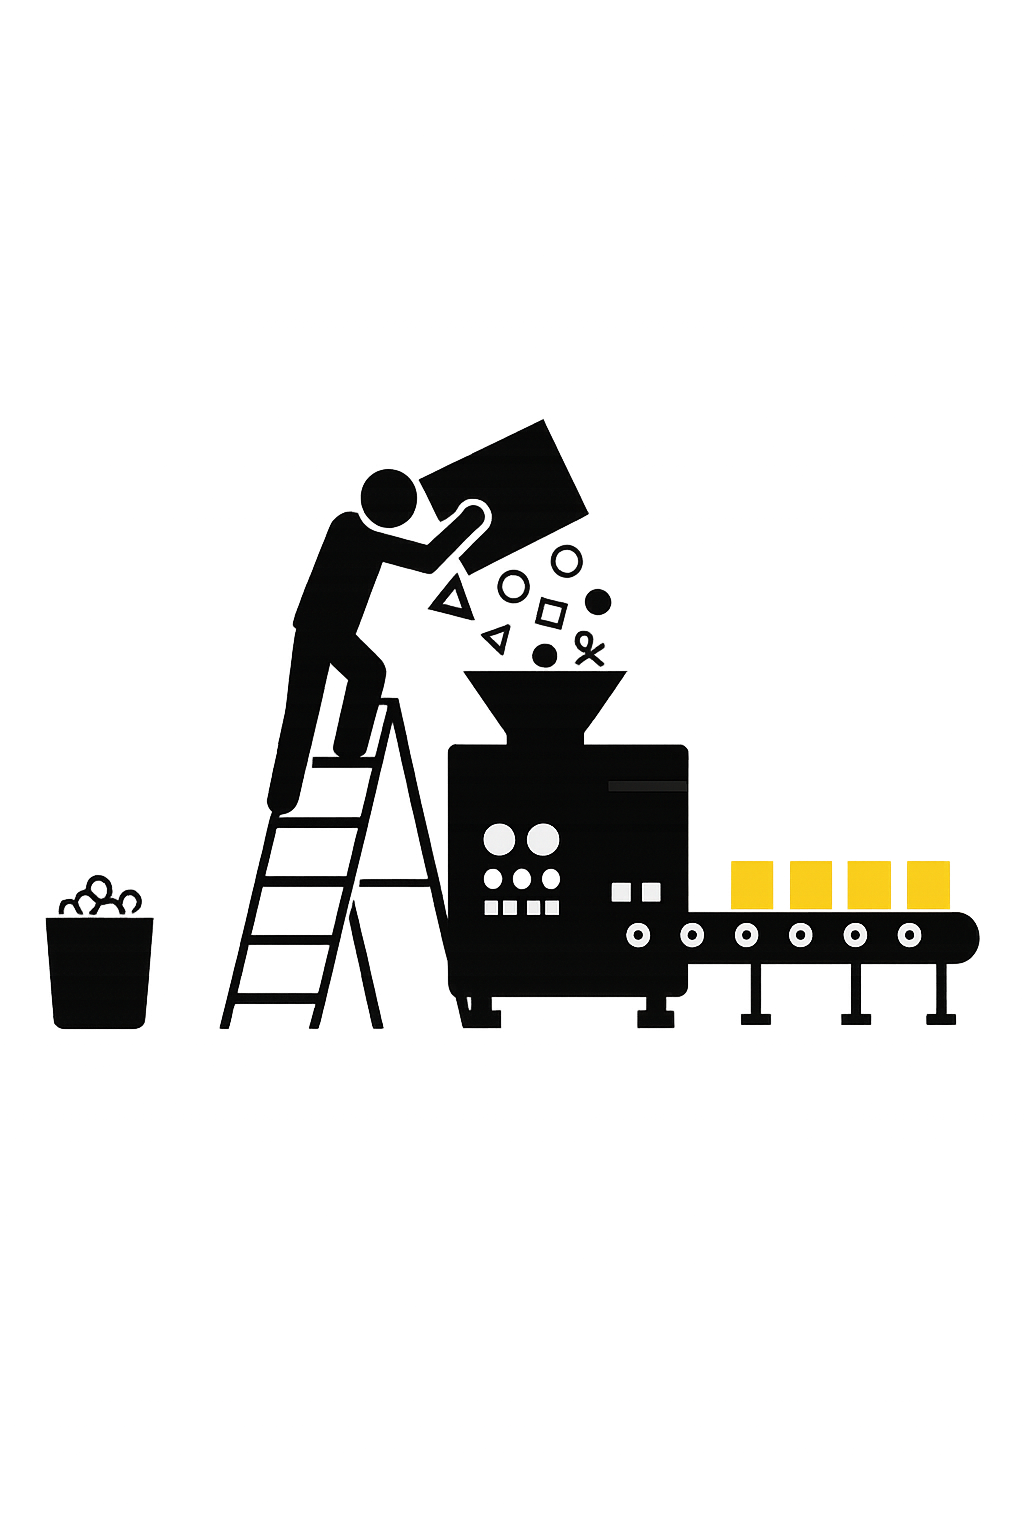
\includegraphics[width=0.5\linewidth]{pics/illustration.png}
    \end{center}

    \newpage

    \tableofcontents
    %\listoffigures
    %\listoftables
    \lstlistoflistings

    \newpage

    %---Document
    \section{Table des identificateurs}

    Dans le cadre de ce projet, nous avons mis en place une structure appelée \texttt{IdentifierTable} destinée à gérer les informations associées à chaque identifiant du programme NILNOVI : variables, constantes, fonctions, procédures, etc.).

    \subsection{Motivations et rôle}
    La table des identificateurs constitue une structure essentielle au compilateur. Elle permet de : 
    \begin{itemize}
        \item mémoriser les caractéristiques des entités déclarées dans le code source, 
        \item garantir l'unicité et la validité des déclarations,
        \item associer chaque identifiant à une adresse mémoire statique, 
        \item résoudre les identifiants lors de la génération du code objet,
        \item réaliser une analyse sémantique
    \end{itemize}

    \subsection{Structure interne}
    Chaque identifiant est représenté par un objet de la classe \texttt{IdentifierCarac}, avec les champs suivants : 
    \begin{itemize}
        \item \texttt{name} : nom de l'identifiant 
        \item \texttt{type} : \texttt{integer}, \texttt{boolean}, \texttt{procedure} ou \texttt{fonction},
        \item \texttt{scope} : \texttt{global}, \texttt{local} ou \texttt{parameter},
        \item \texttt{isIn}/\texttt{isOut} : booléens pour les paramètres,
        \item \texttt{value} : valeur associée 
    \end{itemize}

    \vspace{12pt}
    
    Un compteur d'adresse est maintenu pour chaque portée afin d'attribuer automatiquement une position dans la pile, unique à chaque identifiant lors de son insertion. 

    \subsection{Fonctionnement à la compilation}

    L'ajout d'identifiants dans la table est effectué à l'analyse syntaxique, via des appels comme :
    \begin{lstlisting}[language=python, xleftmargin=20pt]
ident = IdentifierCarac(IdentifierType.INTEGER, "x", scope="local")
id_table.addIdentifier("x", ident)} \end{lstlisting}

    Ainsi, la correspondance entre les identifiants et les emplacements mémoire du programme est assurée de manière fiable et centralisée. 

    \subsection{Affichage et débogage}

    Une méthode \texttt{printTable} permet de visualiser l'état complet de la table, y compris les types, adresses, et valeurs, ce qui peut s'avérer utile pour le développement et le débogage du compilateur.

    \begin{center}
        \begin{tabular}{|l|l|l|l|l|l|l|}
            \hline
            \textbf{name} & \textbf{type} & \textbf{scope} & \textbf{In} & \textbf{Out} & \textbf{address} & \textbf{value} \\
            \hline
            x & integer & global & None & None & 0 & 5 \\
            y & boolean & local & None & None & 0 & None \\
            n & integer & parameter & True & False & 0 & None \\
            \hline
        \end{tabular}
    \end{center}

    \section{Compilateur}

    Dans le cadre de ce projet, nous avons développé une classe \texttt{Compiler} permettant de gérer la génération du code objet de notre analyseur syntaxique.

    \subsection{Classe \texttt{Compiler}}

    La classe \texttt{Compiler} a pour rôle de stocker les instructions générées pendant l'analyse syntaxique. Elle contient une liste d'instructions, \texttt{self.instructions}, dans laquelle sont ajoutées toutes les opérations nécessaires à l'exécution du programme source. Ces instructions sont ajoutées via la méthode \texttt{add\_instruction(name, *args)} qui vérifie que l'instruction est bien définie dans la liste \texttt{compiled\_possible\_instructions}, puis l’ajoute à la séquence.

    Cette classe offre également plusieurs méthodes auxiliaires permettant :

    \begin{itemize}
        \item de connaître l'adresse actuelle dans la mémoire des instructions (\texttt{get\_current\_address}),
        \item de modifier les arguments d'une instruction déjà insérée (\texttt{set\_instruction\_args}),
        \item de gérer les allocations mémoire avec \texttt{new\_identifier} et \texttt{add\_reserver\_instruction},
        \item d'empiler le nombre de paramètres pour les appels de fonctions et procédures avec \texttt{new\_param} et \texttt{add\_trastat\_instruction}.
    \end{itemize}

    \subsection{Intégration dans la classe \texttt{Grammar}}

    La classe \texttt{Grammar}, issue du fichier \texttt{anasyn.py}, contient les règles de grammaire de notre langage. C’est dans cette classe que les appels à \texttt{Compiler} sont effectués aux moments appropriés.

    Par exemple, dans la méthode \texttt{program}, correspondant à la règle $<$program$>$, on insère les instructions \texttt{debutProg} et \texttt{finProg} pour marquer respectivement le début et la fin du programme :

    \begin{lstlisting}[language=python, xleftmargin=20pt]
self.comp.add_instruction('debutProg')
...
self.comp.add_instruction('finProg') \end{lstlisting}

    De même, lors de la déclaration de procédures et fonctions, les instructions \texttt{retourProc} et \texttt{retourFonct} sont ajoutées pour indiquer la fin de leur exécution.

    Cette organisation permet de lier directement la structure syntaxique du langage aux instructions de bas niveau qui seront ensuite interprétées ou traduites.

    \subsection{Conclusion}

    Cette séparation entre la grammaire et la génération du code assure une meilleure modularité du projet. La classe \texttt{Compiler} agit comme un gestionnaire de code objet, tandis que la classe \texttt{Grammar} applique la logique syntaxique et structurelle du langage en déléguant la génération de code à \texttt{Compiler}.

    \newpage

    \section{Machine Virtuelle}

    Cette section présente l'implémentation d'une machine virtuelle (VM) pour l'exécution du code objet généré par le compilateur précédemment décrit pour le langage Nilnovi. Cette VM agit comme un interpréteur capable d'exécuter des instructions de bas niveau représentant des programmes écrits en Nilnovi et Nilnovi procédural.

    \subsection{Architecture Générale}

    Le code de la machine virtuelle Nilnovi est structuré autour de plusieurs composants principaux : la classe VM (cœur de l'interpréteur), la classe Stack (structure de pile avec accès indexé), le système de mémoire (pile d'exécution et tas) basée sur la classe Stack, et le moteur d'exécution (boucle principale d'interprétation).

    La classe \texttt{VM} encapsule l'état complet de la machine virtuelle avec les variables d'état principales : \texttt{stack} (pile d'exécution principale), \texttt{heap} (tas pour l'allocation dynamique), \texttt{base} (pointeur de base pour les blocs d'activation), et \texttt{co} (compteur ordinal/instruction pointer).

    \begin{lstlisting}[caption=Structure principale de la VM,language=python, xleftmargin=20pt]
class VM:
    def debutProg(self):
        self.stack = Stack()
        self.heap = Stack()
        self.base = 0 \end{lstlisting}

    \subsection{Gestion de la Mémoire}

    La classe \texttt{Stack} implémente une pile avec accès indexé, permettant les opérations classiques (\texttt{push()}, \texttt{pop()}, \texttt{summit()}) ainsi que l'accès direct (\texttt{get\_value\_at()}, \texttt{set\_value\_at()}) avec gestion automatique du pointeur de sommet.

    \begin{lstlisting}[caption=Implémentation de la pile,language=python, xleftmargin=20pt]
def push(self, v: Any) -> None:
    self.stack.append(v)
    self.ip += 1

def pop(self) -> Any:
    if self.ip == -1:
        raise ValueError('Cannot pop an empty stack !')
    ret = self.stack[self.ip]
    del self.stack[self.ip]
    self.ip -= 1
    return ret \end{lstlisting}

    La VM utilise un modèle mémoire à deux zones : la pile pour le stockage des variables locales, paramètres et valeurs temporaires, et le tas pour l'allocation dynamique des objets et structures complexes. L'adressage suit le schéma classique avec \texttt{base} comme référence pour les blocs d'activation.

    \subsection{Jeu d'Instructions}

    Le jeu d'instructions de la VM couvre plusieurs catégories d'opérations :

    \subsubsection{Opérations de Base et Mémoire}
    Les opérations de gestion de pile incluent \texttt{reserver(n)} pour réserver n emplacements, \texttt{empiler(val)} pour empiler une valeur, et \texttt{empilerAd(addr)} pour empiler une adresse relative à la base. Les opérations mémoire comprennent \texttt{affectation()} pour affecter une valeur à une adresse et \texttt{valeurPile()} pour déréférencer une adresse.

    \subsubsection{Opérations Arithmétiques et Booléennes}
    La VM supporte l'ensemble des opérations arithmétiques (addition, soustraction, multiplication, division, négation) et booléennes (comparaisons, opérations logiques ET/OU/NON).

    \begin{lstlisting}[caption=Exemple d'opération arithmétique,language=python, xleftmargin=20pt]
def add(self):
    """Addition: pop op2 et op1, push op1 + op2"""
    op2 = self.stack.pop()
    op1 = self.stack.pop()
    self.stack.push(op1 + op2) \end{lstlisting}

    \subsubsection{Instructions de saut}
    Les instructions de saut incluent \texttt{tra(addr)} pour un saut inconditionnel et \texttt{tze(addr)} pour un saut conditionnel si le sommet de la pile est faux. La gestion des adresses tient compte de l'indexation interne avec des ajustements appropriés.

    \subsection{Gestion des Procédures et Fonctions}

    La VM implémente un mécanisme complet de gestion des appels avec \texttt{traStat(a, nbp)} pour les appels statiques, \texttt{reserverBloc()} pour la préparation des blocs d'activation, \texttt{retourProc()} pour le retour de procédure, et \texttt{retourFonct()} pour le retour de fonction avec valeur. Le passage de paramètres est géré via \texttt{empilerParam(ad)} avec calcul d'adresses relatives à \texttt{base}.

    \subsection{Support Orienté Objet}

    La VM supporte les constructeurs d'objets avec \texttt{traConstr(ad, nbP)} pour l'appel de constructeur, \texttt{retourConstr()} pour le retour, et allocation automatique dans le tas. Les opérations sur le tas incluent \texttt{empilerTas(val)}, \texttt{empilerIpTas()} pour récupérer l'adresse courante, et \texttt{empilerAdAt(v)} pour l'accès aux attributs d'objets.

    \subsection{Système de Debug}

    La VM intègre un système de debug à trois niveaux : niveau 0 (aucun debug), niveau 1 (affichage formaté avec état détaillé de la pile, pointeurs, et instruction courante), et niveau 2 (logging avec horodatage). Le mode debug niveau 1 affiche l'état complet de la pile avec marqueurs (TOP, BASE), les valeurs des pointeurs, l'instruction courante avec paramètres, et l'état du tas.

    \subsection{Parsing et Exécution}

    Les instructions Nilnovi suivent le format \texttt{instruction(param1,param2,...)}. La fonction 

    \texttt{parse\_nilnovi\_object\_line()} décompose chaque instruction en séparant le nom de l'instruction et ses paramètres numériques. 

    \begin{lstlisting}[caption=Parsing d'instruction,language=python, xleftmargin=20pt]
def parse_nilnovi_object_line(line: str) -> list[str | int]:
    ret = []
    line = line.strip('\n')
    
    if '()' in line or '(' not in line:
        return [line.strip('()')]
    
    ret.append(line[:line.index('(')])
    arguments_str = line[line.index('(') + 1:line.index(')')]
    args = arguments_str.split(',')
    
    for arg in args: 
        ret.append(int(arg))
    
    return ret \end{lstlisting}

    La boucle d'exécution principale implémente le cycle fetch-decode-execute classique avec gestion des exceptions. L'exécution utilise la réflexion Python pour dispatcher dynamiquement les instructions vers les méthodes correspondantes. Celle-ci nous permet d'éviter d'avoir une boucle principale avec un \texttt{switch} et énormément de \texttt{cases} pour savoir quelle opération appeler.

    \begin{lstlisting}[caption=Dispatch dynamique des instructions,language=python, xleftmargin=20pt]
def execute_instruction(self, instruction):
    nom_instr = instruction[0]
    
    if hasattr(self, nom_instr):
        method = getattr(self, nom_instr)
        if len(instruction) > 1:
            method(*instruction[1:])
        else:
            method()
    else:
        raise ValueError(f"Unknown instruction: {nom_instr}") \end{lstlisting}

    \subsection{Gestion des Erreurs et Performances}

    La VM gère plusieurs types d'erreurs : erreurs de pile (pile vide, débordement), erreurs d'adressage (adresses invalides), instructions inconnues, et erreurs runtime. Les erreurs sont propagées via le système d'exceptions Python avec des messages explicites.

    En termes de performances, l'exécution d'instruction est en $\mathcal O(1)$ pour la plupart des opérations, l'accès mémoire est en $\mathcal O(1)$ grâce à l'indexation directe, et le parsing est en $\mathcal O(n)$ où n est la longueur de l'instruction. Des optimisations possibles incluent le pré-parsing des instructions au chargement et le cache des méthodes fréquemment utilisées.

    \subsection{Limitations et Extensions}

    Les limitations actuelles incluent l'absence de garbage collector automatique, une gestion basique des types, un système d'E/S minimal, et pas de gestion des exceptions utilisateur. Les extensions possibles comprennent le support des nombres flottants, la gestion des chaînes de caractères, un système de modules, une interface de debug interactive, et des optimisations JIT.

    Cette implémentation constitue une base solide pour l'exécution de programmes Nilnovi compilés, avec une architecture modulaire permettant des évolutions futures et un système de debug facilitant le développement et la maintenance.

\end{document}
